%\chapter{Фрагменты исходного кода}\label{appendix-MikTeX-TexStudio}		


\chapter{Реализация метода анализа иерархий (Саати)}
\label{appendix:methodSaati}
Листинг кода метода Саати для выбора наилучшего решения из представленных вариантов по заданным критериям.

\textit{main.py:}
\begin{lstlisting}[breaklines]
import json
import my_math as math

model_tmp_table = {}
text = ''

with open('model2.json') as json_model:
# model can also be a python dictionary
model = json.load(json_model)

text = math.makeSignificanceTable(model_tmp_table, model, text)
text = math.makeOptionMatrixTables(model_tmp_table, model, text)
text = math.makeFinaleMatrix(model_tmp_table, model, text)

answer = model_tmp_table['result']

list_d = list(answer.items())
list_d.sort(key=lambda i: i[1])
last_item = len(list_d)-1

for i in list_d:
print('{0:<10} : {1:^7f}'.format(i[0],i[1]))
text += '{0:<10} : {1:^7f}'.format(i[0],i[1]) + "\n"

print('\nBest item is => {:<20}'.format(list_d[last_item][0]))
text += '\nBest item is => {:<20}'.format(list_d[last_item][0])

f= open("result.txt","w+")

f.write(text)
f.close()

my_math.py:
import numpy as np
import json
import copy

def format_matrix(header, matrix, top_format, left_format, cell_format, row_delim, col_delim, val, kek = False, pos = 0):

if(kek):
header.insert(pos, "")
for i in matrix:
i.insert(pos, "")

table = [[''] + header] + [[name] + row for name, row in zip(header, matrix)]
if(kek):
table_format = [['{:^{}}'] + len(header) * [top_format]] + (len(matrix)  - 2 + val) * [[left_format] + (len(header) - 3) * [cell_format] + ['{}'] + 2 * [cell_format]]
else:
table_format = [['{:^{}}'] + len(header) * [top_format]] + (len(matrix)  - 2 + val) * [[left_format] + len(header) * [cell_format]]
col_widths = [max(len(format.format(cell, 0)) for format, cell in zip(col_format, col))for col_format, col in zip(zip(*table_format), zip(*table))]
return row_delim.join(col_delim.join(format.format(cell, width) 
for format, cell, width in zip(row_format, row, col_widths)) 
for row_format, row in zip(table_format, table))



def makeSignificanceTable(model_tmp_table, model, my_str): # Second level matrix
significance_table = {}
criteria = model['criteria']
for idx1, key1 in enumerate(criteria):
row = []
for idx2, key2 in enumerate(criteria):
row.append(criteria[key1]/criteria[key2])
significance_table[key1] = row

for row in significance_table:
tmp = 1
for j in significance_table[row]:
tmp *= j
tmp = tmp**(1./len(significance_table[row]))
significance_table[row].append(tmp)

tmp = 0
for row in significance_table:
tmp += significance_table[row][len(significance_table[row]) - 1]
check = 0

length = len(list(significance_table.values())[0]) - 1
for row in significance_table:
significance_table[row].append(significance_table[row][length] / tmp)
check += significance_table[row][length + 1]

str = 'Significance Table'
print("\n"+"#"*(6 + len(str))+"\n\n   " + str + "\n\n"+"#"*(6 + len(str)))
my_str += "\n"+"#"*(6 + len(str))+"\n\n   " + str + "\n\n"+"#"*(6 + len(str)) + "\n"
header = [key for key in significance_table]
matrix = [significance_table[key] for key in significance_table]
print(format_matrix(header, matrix, '{:^{}}', '{:<{}}', '{:>{}.5f}', '\n', ' | ', 2))
my_str += format_matrix(header, matrix, '{:^{}}', '{:<{}}', '{:>{}.5f}', '\n', ' | ', 2) + "\n\n\n"

print("\n\n")

model_tmp_table['significance_criteria'] = significance_table
return my_str


def makeOptionMatrixTables(model_tmp_table, model, my_str): # Third level matrixs
matrix = {}
matrix_by_options = model['options']
criteria_names = model['criteria'].keys()
tmp_list = matrix_by_options.values()
length = len(list(tmp_list)[0])	

for i in range(length):
table = []
for idx1, key1 in enumerate(matrix_by_options):
row = []
for idx2, key2 in enumerate(matrix_by_options):
row.append(matrix_by_options[key1][i] / matrix_by_options[key2][i])
table.append(row)

matrix[list(criteria_names)[i]] = table

for idx, key in enumerate(matrix):
table = matrix[key]
for row in table:
tmp = 1
for j in row:
tmp *= j
tmp = tmp**(1./len(row))
row.append(tmp)

for idx, key in enumerate(matrix):
tmp = 0
for row in matrix[key]:
tmp += row[len(row) - 1]
check = 0
length = len(matrix[key][0]) - 1
for row in matrix[key]:
row.append(row[length] / tmp)
check += row[length + 1]

str1 = 'Tables of significant factors for each criterion'
print("\n"+"#"*(6 + len(str1))+"\n\n   " + str1 + "\n\n"+"#"*(6 + len(str1)))
my_str += "\n"+"#"*(6 + len(str1))+"\n\n   " + str1 + "\n\n"+"#"*(6 + len(str1)) + "\n"
header = [key for key in matrix_by_options]

for key in matrix:
print("\n\tBy "+ key)
my_str += "\n\tBy "+ key + "\n"
tmp = 0
for row in matrix[key]:
tmp += row[len(row) - 1]
check = 0
length = len(matrix[key][0]) - 1
for row in matrix[key]:
row.append(row[length] / tmp)
check += row[length + 1]
answ = format_matrix(copy.deepcopy(header) + ["Weight", "% of importance"], copy.deepcopy(matrix[key]) , '{:^{}}', '{:<{}}', '{:>{}.5f}', '\n', ' | ', 2, True, len(header))
print(answ)
my_str += answ + "\n"
print("SUM %: ", check)
my_str += "SUM %: " + str(check) + "\n"
print("\n\n")
model_tmp_table['matrix_by_criteria'] = matrix
return my_str


def makeFinaleMatrix(model_tmp_table, model, my_str): # Final result
final = []
for_multiply = model_tmp_table["significance_criteria"]
conclusion = model_tmp_table["matrix_by_criteria"]

str = 'Final matrix for calculating weights for each element'

fin_answ_tab = "\n"+"#"*(6 + len(str))+"\n\n   " + str + "\n\n"+"#"*(6 + len(str)) + "\n\n"

header = [key for idx, key in enumerate(conclusion)]
str_leng = max([len(key) for idx, key in enumerate(conclusion)])
ttt = max([len(key) for idx, key in enumerate(model['options'])])
str_leng = max(str_leng, ttt)
str_leng =  8 if str_leng<8 else str_leng
side = [key for idx, key in enumerate(model['options'])]
side.insert(0, " " * str_leng)

for i, row in enumerate(side):
if i == 0:
for idx, key in enumerate(conclusion):
row += "|"
row += "{name:<{size}}".format(name=key, size=str_leng)
row += "|" +  "{name:<{size}}".format(name="% weight", size=str_leng) + "\n"
row += "-" * str_leng + "|" + "|".join([("-" * str_leng) for i in range(len(conclusion) + 1)]) + "\n"
else:
row = "{name:<{size}}".format(name=row, size=str_leng)
summ_to_final = 0
for idx, key in enumerate(conclusion):
summ_to_final += copy.deepcopy(conclusion[key][i-1]).pop() * copy.deepcopy(for_multiply[key]).pop()
row += "|" + "{name:>{size}.5f}".format(name=copy.deepcopy(conclusion[key][i-1]).pop(), size=str_leng)

row += "|" + "{name:>{size}.5f}".format(name=summ_to_final, size=str_leng) +"\n" 
fin_answ_tab += row
fin_answ_tab += "-" * str_leng + "|" + "|".join([("-" * str_leng) for i in range(len(conclusion))]) + "|" + "\n"
fin_answ_tab += "{name:^{size}}".format(name="SP", size=str_leng) + "|"
for i, key in enumerate(for_multiply): 
fin_answ_tab += "{name:>{size}.5f}".format(name=copy.deepcopy(for_multiply[key]).pop(), size=str_leng) + "|"

fin_answ_tab += "\n\n\t Where SP - the significance of the criterion\n\n"
print(fin_answ_tab)
for idx, key in enumerate(conclusion):
row = []
length = len(for_multiply[key]) - 1
for i in conclusion[key]:
row.append(i[len(i)-1] * for_multiply[key][length])
final.append(row)

arr1 = np.array(final)
arr1_transpose = arr1.transpose()
okey = {}
x = iter(list(model["options"].keys()))
for i in arr1_transpose:
k = next(x)
okey[k] = sum(i)

model_tmp_table['result'] = okey
return my_str + fin_answ_tab
\end{lstlisting}

\chapter{Расчёт наилучшего транспорта передачи данных} \label{appendix:calculBestTransferDataWay}

Зададим значимость к критерия для расчётов. Количество запросов  на опрос сервера (Cnt req on poll): 4. Количество служебных заголовков вместе с ответом (Cnt of serv head): 3. Служебная информация прикрепляемая в ответе и запросе (Service info): 5. Согласно \taref{comparisonOfTypesOfDataTransmission}, модель соответствия вариантов критериям имеет следующие значения:

\begin{lstlisting}
{
	"name": "Choose transfer data",
	"criteria": { 
		"Cnt req on poll"		: 4,
		"Cnt of serv head"	: 3,
		"Service info"			: 5
	},
	"options": {
		"WebSockets"         :   [4, 4, 5],
		"Server-sent events" :   [4, 4, 4],
		"Long Polling"       :   [4, 3, 2],
		"Ajax Polling"       :   [3, 3, 2]
	} 
}
\end{lstlisting}

Расчёт наилучшего решения приведённой модели из Приложения \ref{appendix:methodSaati}:

\begin{figure}
	\centering
	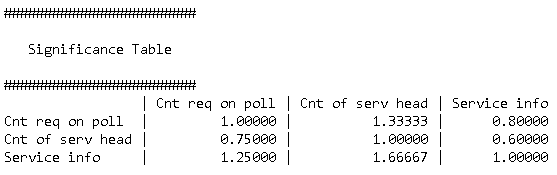
\includegraphics[width=1\linewidth]{my_folder/images/ATransferData1}
	\caption{Таблица значимости}
	\label{fig:atransferdata1}
\end{figure}

\begin{figure}
	\centering
	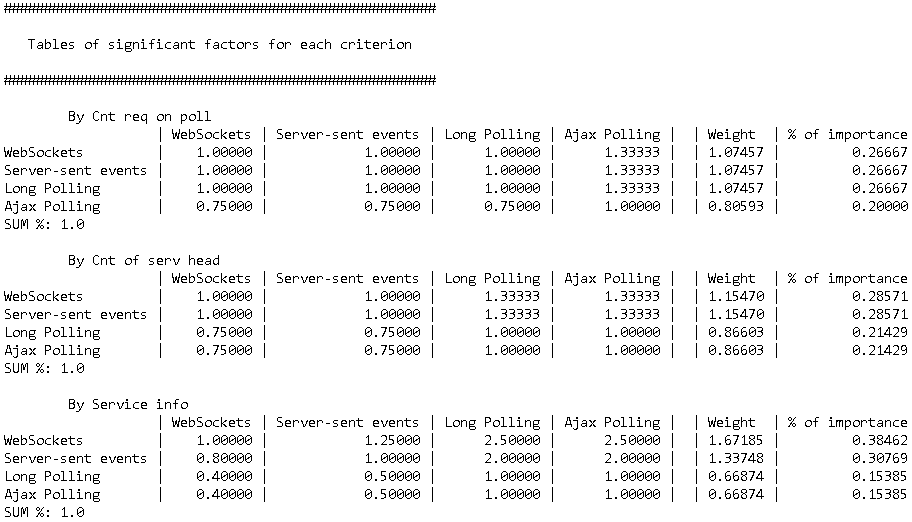
\includegraphics[scale=0.7, angle=270]{my_folder/images/ATransferData2}
	\caption{Таблицы значимых факторов для каждого критерия}
	\label{fig:atransferdata2}
\end{figure}

\begin{figure}
	\centering
	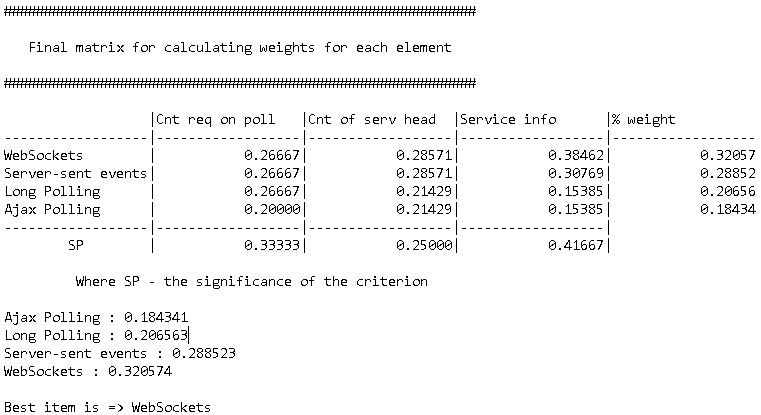
\includegraphics[width=1\linewidth]{my_folder/images/ATransferData3}
	\caption{Результируюящя таблица}
	\label{fig:atransferdata3}
\end{figure}


\chapter{Сравнение выполнения одинаковых задач разными языками программирования}
\label{appendix:comparationPL}

Данная таблица построена на основе данных с электронного ресурса \cite{\ref{appendix:methodSaati}} . Цветовая идентификация имеет следующий характер: Насыщенный зелёный – самый лучший результат, зелёный – второй лучший результат, оранжевый – самый худший результат.

\begin{table}
	\caption{Список угроз с основными методами противодействия им}
	\label{listOfRisk232}
	\centering
	\begin{tabularx}{\linewidth}{p{4.5cm}cccc}
		& PHP & Node js & Java & Python \\
		regex-redux & \cellcolor[rgb]{0.76,0.84,0.61} 2,88 & 9,53 & \cellcolor[rgb]{0.89,0.42,0.04} 10,27 & \cellcolor[rgb]{0.57,0.82,0.31} 2,67 \\
		pidigits & \cellcolor[rgb]{0.76,0.84,0.61} 2,11 & \cellcolor[rgb]{0.89,0.42,0.04} 2,58 & \cellcolor[rgb]{0.57,0.82,0.31}  1,83 & 2,39 \\
		k-nucleotide & 41,32 & \cellcolor[rgb]{0.76,0.84,0.61} 26,32 & \cellcolor[rgb]{0.57,0.82,0.31} 9,14 & \cellcolor[rgb]{0.89,0.42,0.04} 72,58 \\
		binary-trees & 51,13 & \cellcolor[rgb]{0.76,0.84,0.61} 19,22 & \cellcolor[rgb]{0.57,0.82,0.31} 8,28 & \cellcolor[rgb]{0.89,0.42,0.04} 80,82 \\
		reverse-complement & 14,19 & \cellcolor[rgb]{0.76,0.84,0.61} 4,1 & \cellcolor[rgb]{0.57,0.82,0.31} 3,27 & \cellcolor[rgb]{0.89,0.42,0.04} 16,41 \\
		spectral-norm & 33,24 & \cellcolor[rgb]{0.76,0.84,0.61} 4,4 & \cellcolor[rgb]{0.57,0.82,0.31} 4,15 & \cellcolor[rgb]{0.89,0.42,0.04} 170,1 \\
		fannkuch-redux & 219,15 & \cellcolor[rgb]{0.76,0.84,0.61} 19,48 & \cellcolor[rgb]{0.57,0.82,0.31} 16,12 & \cellcolor[rgb]{0.89,0.42,0.04} 494,58 \\
		n-body & 329,52 & \cellcolor[rgb]{0.76,0.84,0.61} 26,28 & \cellcolor[rgb]{0.57,0.82,0.31} 21,85 & \cellcolor[rgb]{0.89,0.42,0.04} 891,12 \\
		fasta & 53,24 & \cellcolor[rgb]{0.76,0.84,0.61} 3,62 & \cellcolor[rgb]{0.57,0.82,0.31} 2,22 & \cellcolor[rgb]{0.89,0.42,0.04} 63,63 \\
		mandelbrot & 105,4 & \cellcolor[rgb]{0.57,0.82,0.31} 6,84 & \cellcolor[rgb]{0.57,0.82,0.31} 6,84 & \cellcolor[rgb]{0.89,0.42,0.04} 263,87 \\
	\end{tabularx}
\end{table}

\chapter{Выбор серверного языка}
\label{appendix:choosingServerSideLanguage}

Зададим значимость к критерия для расчётов. Согласно Таблица \ref{comparisonOfProgrammingLanguage}., модель соответствия вариантов критериям имеет следующие значения:

\begin{lstlisting}
{
	"name": "Choose best language",
	"criteria": { 
		"Libraries"	: 4,
		"DB"				: 3,
		"Speed"			: 5,
		"Framework"	: 4
	},
	"options": {
		"Python"	:   [5, 3, 3, 4],
		"Node Js"	:   [5, 4, 4, 5],
		"Java"		:   [4, 5, 5, 4],
		"PHP"			:   [4, 4, 4, 4]
	} 
}
\end{lstlisting}

Расчёт наилучшего решения приведённой модели с Приложение \ref{appendix:methodSaati}

\begin{figure}
	\centering
	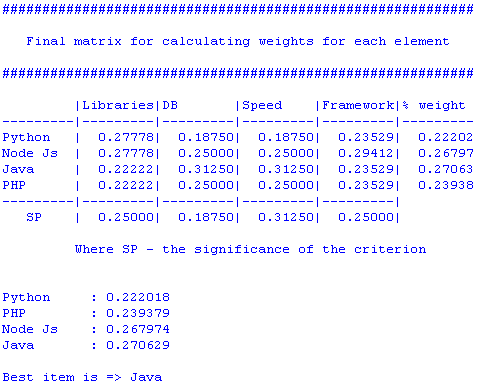
\includegraphics[width=1\linewidth]{my_folder/images/BestSolution1}
	\caption{Результирующая таблица}
	\label{fig:BestSolution1}
\end{figure}

\chapter{Реализация серверной части Socket.io}
\label{appendix:serverSideBySocketIO}

Листинг программного кода серверной части на Node.js, Express.js и Socket.io, для анализа библиотек.


\begin{lstlisting}
const path = require('path');
const express = require('express');

const port = process.env.PORT || 80;
const app = express();
const server = require('http').Server(app); 
const socketio = require('socketio')(server);

const uuid = require('uuid/v4');
const createCsvWriter = require('csv-writer').createObjectCsvWriter; const csvWriter = createCsvWriter({
path: 'stats-si.csv',
header: [
{id: 'msg', title: 'MSG'},
{id: 'id', title: 'UUID'},
{id: 'tmspStart', title: 'TMPSTART'},
{id: 'tmspEnd', title: 'TMPEND'}
] 
});
const messageCount = 1000;
const stats = new Map();

io.on('connection', socket => {
for (let t = 0; t < messageCount; t++) {
const id = uuid();
const sendedMsg = { msg: 'ping', id, tmspStart: Date.now(), tmspEnd: ''};
stats.set(sendedMsg.id, sendedMsg); io.sockets.emit('message', JSON.stringify(sendedMsg));
}

socket.on('message', (message) => {
if (counter < messageCount) {
counter++;
} else {
io.close();
}
const parsedMsg = JSON.parse(message);
parsedMsg.tmspEnd = Date.now();
parsedMsg.msg = "roundtrip";
parsedMsg.tmspStart; stats.set(parsedMsg.id, parsedMsg);
});

socket.on('disconnect', () => {
const records = Array.from(stats, keyValuePair => keyValuePair[1]);
csvWriter.writeRecords(records)
.then(() => {
})
.catch((err) => { console.log(err) });
})
});

app.get('/', function (req, res) {
res.sendFile(path.resolve('../index.html'));
});

server.listen(port, () => console.log(`Listening on port ${port}`));
\end{lstlisting}

\chapter{Реализация серверной части SockJS}
\label{appendix:serverSideBySockJS}

Листинг программного кода серверной части на Node.js, Express.js и Socket.io, для анализа библиотек.

\begin{lstlisting}
const http = require('http');
const sockjs = require('sockjs');
const node_static = require('node-static'); 
const path = require('path'); const fs = require("fs");
const uuid = require('uuid/v4');
const createCsvWriter = require('csv-writer').createObjectCsvWriter; const csvWriter = createCsvWriter({
path: 'stats-sk.csv',
header: [
{id: 'msg', title: 'MSG'},
{id: 'id', title: 'UUID'},
{id: 'tmspStart', title: 'TMPSTART'},
{id: 'tmspEnd', title: 'TMPEND'}
]
});

const sockjs_opts = {
prefix: '/echo'
};

const port = 80;
const messageCount = 1000;
let counter = 0;
const stats = new Map();
const sockjs_echo = sockjs.createServer(sockjs_opts); sockjs_echo.on('connection', function(conn) {
for (let t = 0; t < messageCount; t++) {
const id = uuid();
const sendedMsg = { msg: 'ping', id, tmspStart: Date.now(), tmspEnd: ''};
stats.set(sendedMsg.id, sendedMsg);
conn.write(JSON.stringify(sendedMsg));
}
conn.on('data', (message) => {
if (counter < messageCount) {
counter++;
} else {
conn.close();
}
const parsedMsg = JSON.parse(message);
parsedMsg.tmspEnd = Date.now();
parsedMsg.msg = "roundtrip";
stats.set(parsedMsg.id, parsedMsg);
});
conn.on('close', function() {
console.log('connection is closed');
const records = Array.from(stats, keyValuePair => keyValuePair[1]);
csvWriter.writeRecords(records);
});
});

const static_directory = new node_static.Server(path.resolve('../test-ws/client/index-sk.html'));

const server = http.createServer(); server.addListener('request', function(req, res) {
static_directory.serve(req, res);
});

server.addListener('upgrade', function(req, res) { 
res.end();
});
sockjs_echo.installHandlers(server);
console.log(` Server listening on ${port}`);
server.listen(port, hostname);

\end{lstlisting}


\chapter{Выбор систему мониторинга}
\label{appendix:choosingMonitoringSys}

Зададим значимость к критерия для расчётов. Согласно Таблица \ref{comparisonOfAPM}., модель соответствия вариантов критериям имеет следующие значения:


\begin{lstlisting}
{
  "name": "Choose best APM",
  "criteria": { 
    "UI"                             : 3,
    "Distribution"                   : 4,
    "Tracing transaction"            : 5,
    "Correlation data"               : 3,
     "Support"                        : 4
  },
  "options": {
    "New Relic"     :   [5, 3, 4, 5, 5],
    "CloudWatch"    :   [3, 4, 1, 3, 3],
    "Dynatrace APM" :   [4, 5, 5, 5, 4],
    "AppDynamics"   :   [5, 5, 4, 4, 5],
    "CA APM"        :   [4, 5, 4, 5, 4]
 } 
}
\end{lstlisting}

Расчёт наилучшего решения приведённой модели с Приложение \ref{appendix:methodSaati}:

\begin{figure}
	\centering
	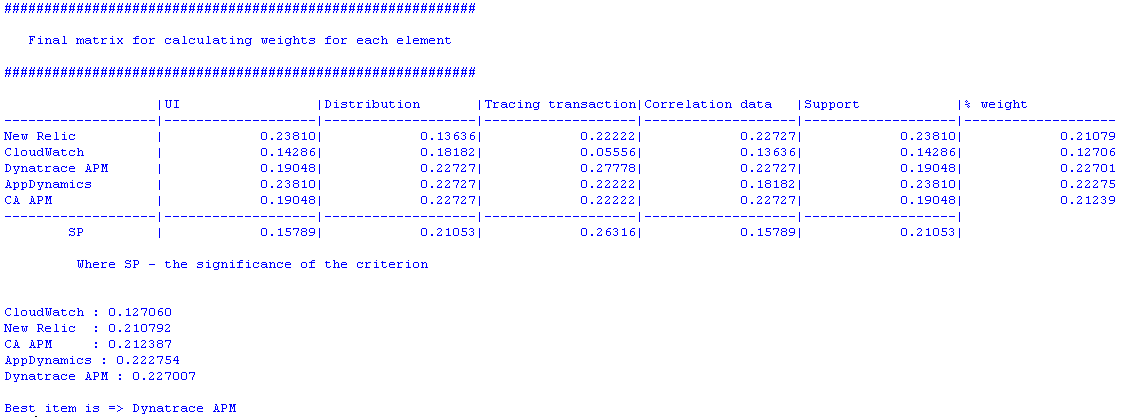
\includegraphics[width=1\linewidth]{my_folder/images/FMatrixMonitoringSys}
	\caption{Результирующая таблица}
	\label{fig:FMatrixMonitoringSys}
\end{figure}


\chapter{Компонента Map (граф)}
\label{appendix:RGTMapGraph}

Листинг кода реализации компоненты Map (граф начального пути яхты в start report)

\begin{lstlisting}
const MyMap = ({ graph, title, angle }) => {
const { classes } = useStoreState(state => state.classes);
const { rawData } = useStoreState(state => state.data);
const [lastZoom, changeLastZoom] = useState(0);
let heap = 0;
const mapRef = useRef(null);

const hideAndSeek = event => {
  let map = event.target;
  heap = 0;
  var zoom = map.getZoom();
  if (zoom < 16 && (!lastZoom || lastZoom >= 16)) {
    map.eachLayer(function(l) {
      if (l.getTooltip()) {
        var tooltip = l.getTooltip();
        l.unbindTooltip().bindTooltip(tooltip, {
          permanent: false
        });
      }
    });
  } else
  map.eachLayer(function(l) {
    if (l.getTooltip()) {
      var tooltip = l.getTooltip();
      l.unbindTooltip().bindTooltip(tooltip, {
        permanent: labelPermanent(tooltip.options.elevation, zoom)
      });
    }
  });

  changeLastZoom(zoom);
};

const labelPermanent = (wheight, zoom) => {
  let denominator = zoom - 16;
  let border = 320 / Math.pow(2, denominator);
  if (heap + wheight > border) {
    heap = 0;
    return true;
  } else {
    heap = heap + wheight;
    return false;
  }
};

const log = num => {
  return Math.log(num) / Math.log(2.0154);
};

const takeZoomLvl = () => {
  let zoomLvl = {
    x: [Math.min(...graph.x), Math.max(...graph.x)],
    y: [Math.min(...graph.y), Math.max(...graph.y)]
  };
  let y = Math.abs(zoomLvl.y[1] - zoomLvl.y[0]);
  let x = Math.abs(zoomLvl.x[1] - zoomLvl.x[0]);
  return Math.min(log(720 / x), log(360 / y));
};
return (
  <>
  {graph.hasOwnProperty("myGeoJSON") &&
  graph.hasOwnProperty("myGeoJSONLable") ? (
    <>
      <Legend />
      <Graphtitle tws={graph.tws} />
      <Arrow angle={angle} />
      {title && <Title title={title} />}
      <Map
        className={classes.mapLeaflet}
        id="leaflet-map"
        center={[graph.center[1], graph.center[0]]}
        useFlyTo={true}
        boundsOptions={{ padding: [25, 25] }}
        zoom={takeZoomLvl()}
        attributionControl={true}
        zoomControl={true}
        doubleClickZoom={true}
        scrollWheelZoom={true}
        dragging={true}
        maxZoom={20}
        minZoom={1}
        animate={true}
        easeLinearity={0.35}
        onZoomend={e => hideAndSeek(e)}
        ref={mapRef}
      >
        <TileLayer url="http://{s}.tile.osm.org/{z}/{x}/{y}.png" />
        {graph.geoJsonLines.features.map((feature, idx) => (
          <GeoJSON
            key={feature.key}
            data={feature}
            style={getStyle(feature.properties.name)}
          >
            {feature.properties.hasOwnProperty("point") ? (
              feature.properties.point.name.map((name, jdx) => (
                <Marker
                  position={feature.properties.point.coordinates[jdx]}
                  key={"SL-" + feature.properties.point.name[jdx]}
                >
                  <Tooltip
                    key={
                      "Tooltip-" + feature.properties.point.name[jdx] + jdx
                    }
                    direction="right"
                    offset={[-25, 15]}
                    elevation={feature.properties.point.elevation}
                    className={"tooltopSP"}
                    permanent={labelPermanent(
                    feature.properties.point.elevation,
                    takeZoomLvl()
                    )}
                  >
                    {feature.properties.point.name[jdx]}
                  </Tooltip>
                </Marker>
              ))
              ) : (
               <></>
              )}
          </GeoJSON>
        ))}
        {graph.myGeoJSON.features.map((feature, idx) => (
          <GeoJSON
            key={"lb- " + idx}
            data={feature}
            style={getStyle("black")}
          />
        ))}
        {graph.myGeoJSON.features.map((feature, idx) => (
          <GeoJSON
            key={"lf-" + idx}
            data={feature}
            style={getStyle(feature.properties.elevation)}
          />
        ))}
        {graph.myGeoJSONLable.map((feature, idx) => (
          <Marker position={feature.coordinates} key={"Marker-" + idx}>
            <Tooltip
              key={"Tooltip-" + idx}
              direction="right"
              offset={[-15, 20]}
              elevation={feature.elevation}
              className={colorTooltip(feature.event)}
              permanent={labelPermanent(feature.elevation, takeZoomLvl())}
            >
              {`${feature.name} ${feature.event}`}
            </Tooltip>
          </Marker>
        ))}
      </Map>
    </>
  ) : (
    <NoData />
  )}
  </>
 );
};

export default MyMap;

\end{lstlisting}

\chapter{Компонента Table}
\label{appendix:RGTTableGraph}

Листинг кода реализации компоненты формирования таблиц реализуемых в приложении.

\begin{lstlisting}
export const DataTable = ({ title, headers, rows, cellClass }) => {
  const { classes } = useStoreState(state => state.classes);

  return (
    <>
      {title && <Title title={title} />}
      {headers.length > 0 && rows.length > 0 ? (
        <div className={classes.tableDiv}>
          <Table className={classes.table}>
            <TableHead>
              <TableRow>
                {headers.map((header, idx) => (
                  <TableCell
                    className={classes.tableHead}
                    key={`header-${idx}`}
                  >
                    {header.trim()}
                  </TableCell>
                ))}
              </TableRow>
            </TableHead>
            <TableBody>
              {rows.map((row, i) => (
                <TableRow
                  key={`row-${i}`}
                  style={{
                    backgroundColor: `${
                      row.hasOwnProperty("Event")
                        ? getColorOfEvent(row.Event)
                        : "white"
                    }`
                  }}
                >
                  {Object.values(row).map((column, j) => (
                    <TableCell
                      style={{
                        borderBottom: `${i === rows.length - 1 &&
                          "2px solid black"}`,
                        backgroundColor: `${column !== null &&
                          column.hasOwnProperty("color") &&
                          column.color}`
                      }}
                      className={cellClass ? cellClass : classes.cell}
                      key={j}
                    >
                      {column === null
                        ? ""
                        : column.hasOwnProperty("percentage")
                        ? column.percentage
                        : column}
                    </TableCell>
                  ))}
                </TableRow>
              ))}
            </TableBody>
          </Table>
        </div>
      ) : (
        <NoData />
      )}
    </>
  );
};

export default DataTable;
\end{lstlisting}

\chapter{RESTful API для /api/start-report}
\label{appendix:ReliseRESTfulAPI}

Реализация RESTful API для конечной точки (endpoint) /api/ start-report

\begin{lstlisting}
const express = require('express');
const router = express.Router();
const User = require('../../db/user');
const formidable = require('formidable');

router.get('/', function(req, res, next) {
  listM = [];
  User.teamList().then(list => {
    for(let i = 0; i < list.length; i++){
      listM.push(JSON.parse(list[i].file));
    }
    console.log(listM);
    if (!isNaN(req.query.id)) {
      User.getOne(req.query.id).then(user => {
        if (user) {
          //console.log(user);
          user = user.pop();
          //console.log(user);
          res.render('index', { title: 'Start report', menuLi: 0, Udata: user, list: listM });
        } else {
          resError(res, 404, "User Not Found");
        }
      });
    } else {
      res.render('index', { title: ''Start report ', menuLi: 0, Udata: false, list: listM });
    }
  });
});

router.post('/addfile*', function(req, res, next) {
  var form = new formidable.IncomingForm();
  form.parse(req, function (err, fields, files) {
    if (!isNaN(req.query.id)) {
      User.getOne(req.query.id).then(user => {
        if (user) {
          //console.log(user);
          user = user.pop();
          console.log(user, fields.team, JSON.stringify(fields.team));
          User.setteam(user, JSON.stringify(fields.team)).then(tt => {
            setTimeout(()=>{res.redirect("/");},150);
          });
        } else {
          resError(res, 404, "User Not Found");
        }
      });
    } else {
      setTimeout(()=>{res.redirect("/");},150);
    }
  });
});

function resError(res, statusCode, message) {
  res.status(statusCode);
  res.json({message});
}

module.exports = router;
\end{lstlisting}